\documentclass[twocolumn,11pt]{abst}



% タイトル
\title{研究室内の環境改善による作業効率の向上}
\author{深澤椋(指導教員 伊藤恒平 林道大)}

%\urlstyle{rm}

\setcounter{page}{31}
\lhead{}
\chead{}
\rhead{{\sf 17・216}\\{\bf 機械工学科}}
\lfoot{}
%\cfoot{{\sf-\ M-\thepage \ -}}
\cfoot{
 \ifnum \value{page} < 10
  {\sf-\ M-0\thepage \ -}
 \else%
  {\sf-\ M-\thepage \ -}
 \fi%
}
\rfoot{}
\renewcommand{\headrulewidth}{3pt}
%\renewcommand{\footrulewidth}{1pt}



\begin{document}

%\layout
\maketitle
\thispagestyle{fancy}
\pagestyle{fancy}

\setlength{\baselineskip}{5.6truemm}
\kanjiskip=.07zw plus 3pt minus 3pt
\xkanjiskip=.07zw plus 3pt minus 3pt


\section{はじめに}
\subsection{研究の背景}
本研究室は,NHK高専ロボコンの地区優勝を目的として活動していたが,一回戦敗退だった.
大会後,反省会のなかで,ロボット製作の遅れこそが最大の要因とし,
次期ロボコン研究室生が次のロボコンで好成績を残すために,製作の遅れを
防止するための措置を行うこととした.

\subsection{研究目的}
製作の遅れ防止として,私は研究室の環境整備こそが
大きな助けとなると考えた.
そこで,より使いやすく,速やかに作業を行える環境を作り出すための室内の模様替えを行い,
研究室を使う上での簡単なルールを設定する.


\section{現状分析}
\subsection{現状把握}
より良い環境作りの為に,現状把握を行う.
参考文献\cite{toyota}やインターネットを用いた調査によって得られた
知識や工夫から,当研究室の問題点をいくつか発見した.
\par 発見した問題点をいかに示す.

\begin{itemize}
\item ネジや部品が取り出しにくい
\item 工具に定位置が決まっていない(または無視されている)ため,
探す必要があるなど余計な時間がかかる
\item 板材の取り出しに時間がかかる
\item 研究に必要ない物(前年のロボットや使わない備品)が多い
\end{itemize}

\subsection{具体的な改善案}
上述した問題点から,次の手順によって研究室内の環境改善を目指す.
\begin{enumerate}
\item 研究に必要のない物,すぐに使い道の浮かばない物,また廃材や古いロボットなどを
解体・廃棄しスペースを作る
\item 新しく,現状より効率よく材料や工具を管理を収納・管理するための棚などを作成する
\item 空いたスペースを利用し,物の配置換えを行う
\item 材料,工具を新しい棚に移して古い棚を廃棄し,新しい棚を配置する
\item 改善した環境を維持するためのルールを設定する
\end{enumerate}

\section{改善内容}
環境改善として,研究室内の掃除,模様替えを行い,工具・材料の新しい収納方法として,
新しいアイテムを作成した.
各改善内容を次に示す.

\subsection{新しい材料収納方法}
従来の材料の収納方法は図\ref{material}のようになっており,この状態では,材料(特に板材)が
取り出しにくい.さらに,棒材が別の棚にも入っている.
そのため,目的の材料を取り出すまでに時間がかかったり,取り出すこと自体に苦労する.
そこで,図\ref{newmaterial}の新しい材料収納棚を作成した.これは,今まで材料を収納していた
棚よりも大きく,また,板材を定尺と使いかけとで分けるなど,収納効率を大幅に向上させるた.

\begin{figure}[htbp]
  \begin{center}
   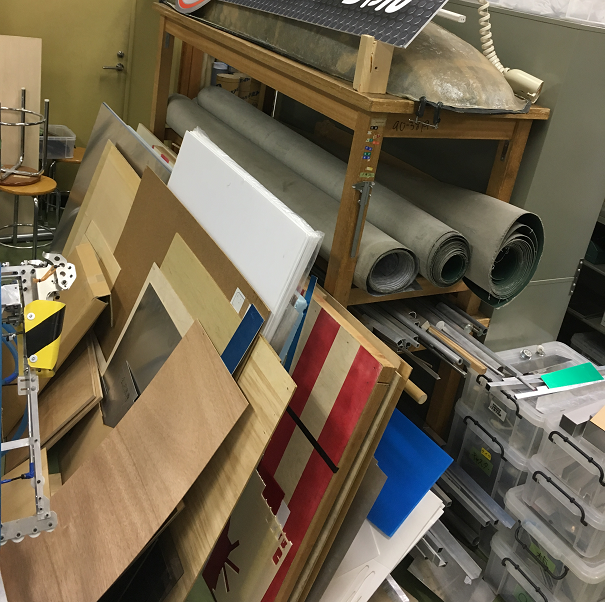
\includegraphics[width=52mm]{materials.png}
  \end{center}
 \caption{従来の収納方法}
\label{material}
\end{figure}

\subsection{新しい工具の管理方法}
今までの工具管理方法は,箱に入れて棚に収めるというものだった.
しかし,この方法では,箱を取り出して蓋を開け,目的の工具を出し箱を戻す
という過程が非効率的だ.
そこで,図\ref{tooldesk}のツールデスクを作成した.これは,直立する有孔ボードに直接
工具を掛けることで,取出・片づけを簡潔にし,さらにどこに何があるのか見つけ
やすいようになっている.

\begin{figure}[htbp]
  \begin{center}
   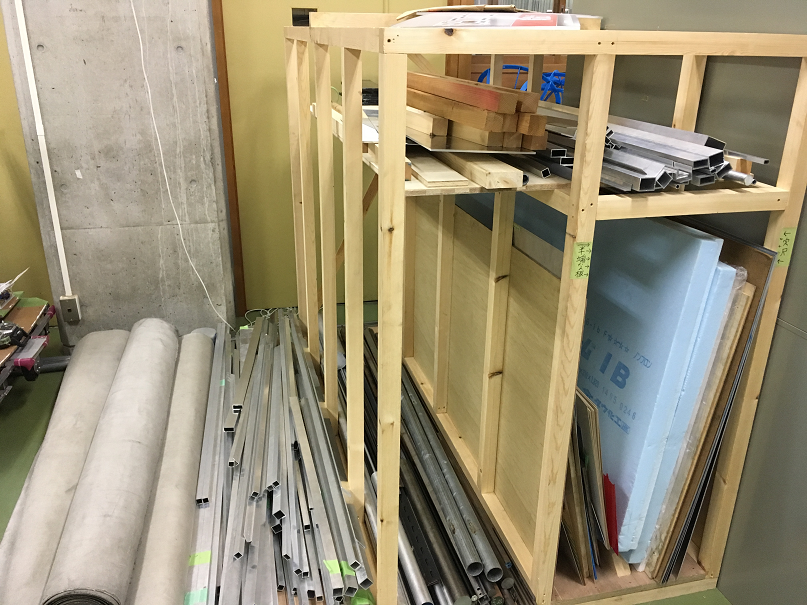
\includegraphics[width=60mm]{newmaterial.png}
  \end{center}
 \caption{新しい収納方法}
\label{newmaterial}
\end{figure}

\begin{figure}[htbp]
  \begin{center}
   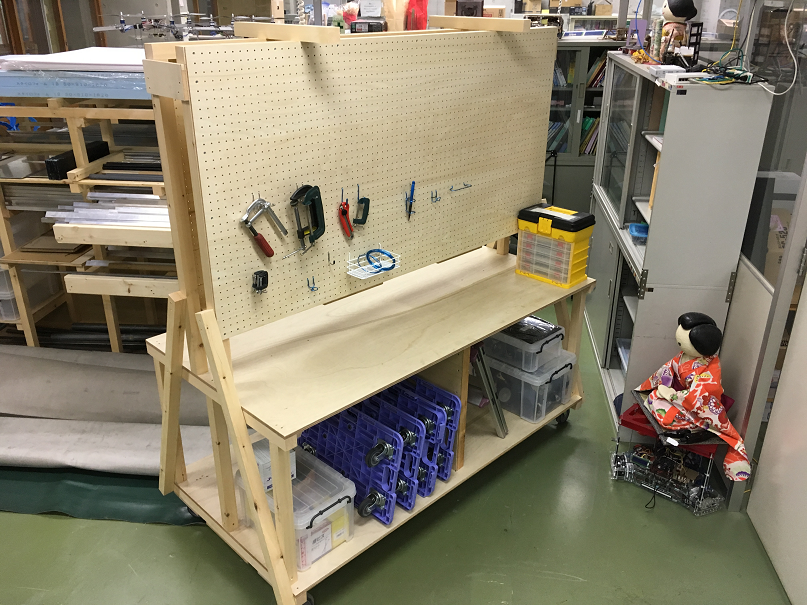
\includegraphics[width=60mm]{tooldesk.png}
  \end{center}
 \caption{ツールデスク}
\label{tooldesk}
\end{figure}


\subsection{模様替え}
模様替え前後の簡単な見取り図を示す。
%模様替え前後の見取り図
\begin{figure}[htbp]
  \begin{center}
   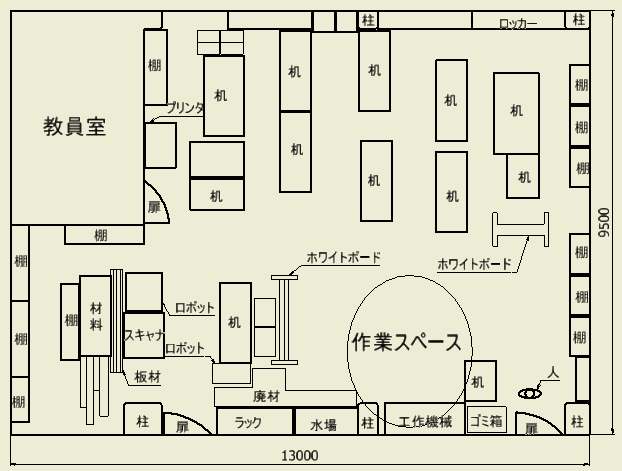
\includegraphics[width=65mm]{beforcad.png}
  \end{center}
 \caption{模様替え前の見取り図}
\label{befor}
\end{figure}

\begin{figure}[htbp]
  \begin{center}
    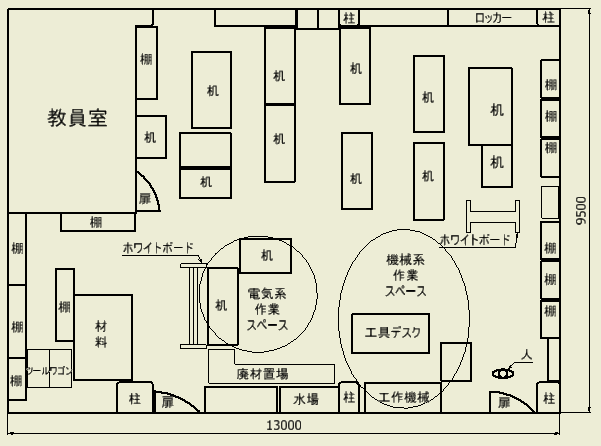
\includegraphics[width=65mm]{aftercad.png}
    \end{center}
  \caption{模様替え後の見取り図}
 \label{after}
\end{figure}
%意図
\par 模様替えは以下の意図をもってを行った。
\begin{itemize}
\item 系統ごとに作業スペースを設けることで,別系統の作業者同士の接触や,
系統違いの工具の混同を防止する
\item あまり使っていなかった扉付近の机を電気系専用の作業机にすることで電気系作業に専念
しやすくした
\item ツールワゴンやホワイトボードを作業スペースの外側に置くことで
空間を確保した
\item ツールデスクを作業スペースに置くことで、工具をすぐに取り出せるようにした
\end{itemize}


\section{新しいルール}
改善された環境を維持するために新しいルールを設定する.
\begin{itemize}
\item 目に見えない場所に物を置かない
\item 使用の目途が立たない物は即廃棄
\item 今あるものから使う
\item 工具の定位置を勝手に変えない
\item 必要以上の発注をしない
\item 使ったら元の位置に戻す
\end{itemize}

\section{今後の課題}
本研究では,時間と労力の問題から,本来何度も行われるべき「検討~実施」過程を一度しか
行っていないため,完成度が高いとは言えない.より高精度な改善を施すには,一年ごとに
フィードバックを行い,その都度改善を行っていく必要がある.

\begin{thebibliography}{2}
\bibitem{toyota} トヨタの片づけ・OJTソリューションズ・(株)KADOKAWA
\end{thebibliography}


\end{document}